\chapter{.NET Framework (40)}

.NET Framework to współczesna platforma aplikacyjna dla systemów rodziny Windows. Wnosi całe mnóstwo nowoczesnych języków i technologii wytwarzania aplikacji. 
Również coraz większa część systemu operacyjnego jest obecnie dostarczana w postaci kodu celującego w środowisko .NET.

Rozwiązanie zadań w tym zestawie polega na napisaniu programów w językach platformy .NET. 
Jeśli nie jest to podane jawnie, sugerowanym językiem jest C\#. 

\section{Podsystem Windows Forms (9)}

\subsection{Podstawowy interfejs użytkownika (1)} 

    Powtórzyć w Windows Forms zadanie według specyfikacji \ref{okno_dialogowe} ze str.\pageref{okno_dialogowe}.

      [{\bf 1p}]  
	
\subsection{Komponenty dodatkowe (1)} 

    Powtórzyć w Windows Forms zadanie według specyfikacji \ref{common_controls} ze str.\pageref{common_controls}.
	{\em Uwaga!} Komponenty pochodzą z podsystemu Windows Forms.

      [{\bf 1p}]  
	
\subsection{Podsystem {\tt GDI+} (2)} 
    Przedstawiony w skrypcie program rysujący w oknie bieżący czas przerobić na wzór zegarka systemowego
\label{podsystem_gdi}	
      Windows, to znaczy tak, żeby bieżąca godzina była przedstawiana na tarczy zegara analogowego a nie cyfrowego.
      
      Wykorzystać funkcje do rysowania z GDI+. 

      [{\bf 2p}]  
      
\subsection{Własny formant (1)}
      
      Zaimplementować własny komponent {\tt SmoothProgressBar}, który
\label{smooth_progress}	  
      będzie imitować zachowanie standardowego komponentu {\tt ProgressBar} (pasek postępu).
      
      Komponent powinien mieć co najmniej 3 propercje: {\tt Min}, {\tt Max} i {\tt Value}, 
      pozwalające określić odpowiednio minimalną, maksymalną i bieżącą wartość paska postępu.      
      Mając te informacje, {\tt SmoothProgressBar} w zdarzeniu {\tt Paint} powinien rysować gładki 
      (w przeciwieństwie do oryginalnego, który jest złożony z "kafelków")
      pasek postępu o odpowiedniej długości (według zadanych proporcji). 
      
	\begin{figure}
	\begin{center}
	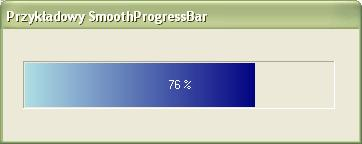
\includegraphics[width=0.6\textwidth]{z6_pb}
	\end{center}
	\caption{Przykładowy {\tt SmoothProgressBar}}
	\end{figure}
      
      [{\bf 1p}]  
	        
\subsection{Pomoc kontekstowa (2)}

    W dowolny sposób przygotować plik pomocy kontekstowej w formacie CHM. 
\label{pomoc_kontekstowa}	
    
    Następnie przykładową aplikację rozszerzyć o obsługę
    pomocy kontekstowej. Należy pokazać, że dla różnych formantów 
    interfejsu użytkownika, przywołanie pomocy kontekstowej przywołuje
    właściwy temat pliku pomocy.
    
    Wskazówki: 
	
	\begin{itemize}
	\item jednym z narzędzni umożliwiających wytworzenie pliku CHM jest darmowy HTML Help Workshop
	\item do wiązania formantów z tematami pomocy można
    użyć bibliotecznego komponentu {\tt HelpProvider} lub jego alternatyw
    w rodzaju 
	
	{\tt http://netpl.blogspot.com/2007/08/con\-text-help-made-easy-reloaded.html}
	\end{itemize}
    
    [{\bf 2p}]  

\subsection{Wykonywanie zadań w tle (1)}

	Zademonstrować w praktyce działanie klasy {\tt BackgroundWorker} oraz jej zdarzenia {\tt ProgressChanged} do delegowania długiego zadania
	do przetwarzania w tle. 
	
	Formalnie - wątek w tle niech testuje jakiś zakres liczb na przykład testem pierwszości. Zakres dobrać tak, aby obliczenia trwały nie krócej niż kilka sekund.
	Postęp obliczeń powinien być raportowany w interfejsie użytkownika za pomocą formantu paska postępu.
	
	Porównać to z zadaniem w tle wykonanym za pomocą standardowego wątka (obiekt {\tt Thread}) który w trakcie obliczeń również aktualizuje pasek	
	postępu obliczeń. Jaka trudność pojawia się w tym drugim podejściu (jest to również odpowiedź na pytanie co wnosi {\tt BackgroundWorker}
	w stosunku do takiego naiwnego podejścia)?

    [{\bf 1p}]  
	
\subsection{Async/await (1)}

	Zaprezentować na niewielkim przykładzie zastosowanie rozszerzeń języka w obszarze programowania asynchronicznego ({\tt async/await}).
	
	Bardziej formalnie - pokazać że w aplikacji okienkowej użycie nieblokującej metody asynchronicznej {\tt HttpClient::ReadStringAsync} 
	do pobrania zawartości z zewnętrznego zasobu sieciowego nie spowoduje zablokowania wątka głównego aplikacji, w którym przetwarzana jest pętla
	obsługi komunikatów. W tej samej aplikacji zademonstrować synchroniczne, blokuące wywołanie metody {\tt WebClient::DownloadString}.
	
    [{\bf 1p}]  

\section{Podsystemy WPF/Metro (4)}

\subsection{Podstawowy interfejs użytkownika (2)} 

    Powtórzyć w WPF zadanie według specyfikacji \ref{okno_dialogowe} ze str.\pageref{okno_dialogowe}.

    [{\bf 2p}]  

\subsection{Komponenty dodatkowe (2)} 

    Powtórzyć w WPF zadanie według specyfikacji \ref{common_controls} ze str.\pageref{common_controls}.
	{\em Uwaga!} Komponenty pochodzą z podsystemu WPF.

    [{\bf 2p}]  
	
 
\section{Biblioteka standardowa .NET (15)}

    Biblioteka standardowa platformy .NET bardzo szybko się rozwija. Współcześnie obejmuje właściwie większość możliwych aspektów technologicznych, przez różne
	podsystemy interfejsu użytkownika, podsystemy graficzne, usługi sieciowe, systemy plików, podsystemy kryptograficzne, usługi kolejkowe i katalogowe, komunikację z systemami
	relacyjnych i nierelacyjnych baz danych oraz programowanie serwerów aplikacyjnych. Jest to ogromny i fascynujący świat, który ma to do siebie, że obojętnie jak dobrze się go zna,
	zawsze można znaleźć tu coś nowego i zajmującego.

	Z uwagi na ograniczone ramy czasowe, przegląd biblioteki standardowej ma tu charakter wybiórczy. 
	
	Ponieważ w przyszłych wersjach systemu operacyjnego Windows interfejs BCL ma szansę
	  stać się natywnym interfejsem programowania Windows, warto szczegółowo zapoznać się z jego możliwościami.
      
\subsection{Własna kompletna klasa usługowa (1)}
      Napisać klasę do obsługi liczb zespolonych. Dodać odpowiednie konstruktory, przeciążyć odpowiednie operatory.
\label{liczby_zespolone}
      
      Rozszerzyć tę klasę o własne formatowane. Ściślej, zaimplementować interfejs
      {\tt IFormat\-table} i obsługiwać dwa rodzaje formatowania:
      \begin{itemize}
      \item domyślne (brak formatowania lub {\tt d}) powinno dawać wynik $a+bi$ 
      \item wektorowe (format {\tt w}) powinno dawać wynik $[a,b]$.
      \end{itemize}
      
      Przykładowy kawałek kodu:
      \begin{verbatim}
      Complex z = new Complex( 4, 3 );
      Console.WriteLine( String.Format( "{0}", z ) );
      Console.WriteLine( String.Format( "{0:d}", z ) );
      Console.WriteLine( String.Format( "{0:w}", z ) );
      \end{verbatim}

      powinien dać wynik

      \begin{verbatim}
      4+3i
      4+3i
      [4,3]
      \end{verbatim}

      [{\bf 1p}]  
                
\subsection{Własna kolekcja danych (1)}
      
      Zaimplementować niegeneryczną kolekcję {\tt Set} działającą jak zbiór, odrzucający duplikaty elementów.
\label{wlasne_kolekcje}	  
      
      {\em Wskazówka: są trzy możliwości - albo dziedziczenie jakiejś kolekcji bibliotecznej, albo zaimplementowanie własnej kolekcji, która wewnętrznie będzie wykorzystywała
      jakąś kolekcję biblioteczną, wreszcie zaimplementowanie własnej kolekcji nie dziedziczącej z żadnej kolekcji bibliotecznej ani nie wykorzystującej wewnętrznie żadnej
      kolekcji bibliotecznej. Ta ostatnia możliwość ma niewielki sens - należy uczyć się korzystania z biblioteki standardowej i wykorzystywać jej komponenty we własnym kodzie,
      a nie wyważać otwarte drzwi implementując już istniejące mechanizmy samemu.}

      [{\bf 1p}]  

\subsection{Składanie strumieni (1)}

      Napisać program, który zawartość wskazanego pliku tekstowego zapisze do {\bf zaszyfrowanego} algorytmem AES {\bf skompresowanego} 
\label{skladanie_strumieni}	  
	  strumienia GZip.
      
      Napisać kolejny program, który odszyfruje wskazany skompresowany strumień GZip.
            
      [{\bf 1p}]

\subsection{Golibroda w .NET (2)}

      Napisać konsolowy program, który rozwiązuje klasyczny problem golibrody lub problem "palaczy tytoniu" 
\label{golibroda_net}	  
      za pomocą którejkolwiek z metod synchronizacji wątków udostępnianej przez .NET BCL.  

      [{\bf 2p}] 
      
\subsection{Protokoły sieciowe (1)}

    Zademonstrować działanie klas {\tt FtpWebRequest}, {\tt HttpWebRequest}, 
	{\tt WebClient}, {\tt HttpClient}, {\tt HttpListener},
\label{protokoly_sieciowe}	
    {\tt TcpListener}, {\tt TcpClient}, {\tt SmtpClient}.
	
	Zwrócić uwagę na te funkcje z interfejsów powyższych klas, których metody pobierania danych są zaimplementowane jako asynchroniczne (zwracają {\tt Task<T>}).

    [{\bf 1p}]

\subsection{Serializacja i przesyłanie obiektów (2)}

    Wybrać jeden z omawianych sposobów serializacji (binarne, XML, SOAP) i przygotować dwa moduły: klienta i serwera.
	
	Klient serializuje wskazany obiekt z danymi (jakaś współdzielona prosta klasa) i przesyła go do serwera. Serwer deserializuje obiekt i zapamiętuje go w pliku.
	
	{\em Wskazówka}. Do implementacji komunikacji klient-serwer można użyć klas 
    {\tt TcpClient} i {\tt TcpListener}) .
    
    [{\bf 2p}]

\subsection{Komunikacja międzyprocesowa - MSMQ (2)}

    Korzystając z MSMQ ({\tt System.Messaging}) utworzyć
\label{msmq}	
    dwukomponentowy system, w którym jeden z komponentów będzie
    co pewien czas tworzył dużą liczbę komunikatów, a drugi komponent
    będzie regularnie opróżniał kolejkę komunikatów, wykonując dla
    każdego z nich jakąś kilkusekundową akcję.
    
    [{\bf 2p}]

\subsection{Globalizacja (1)}

    Napisać program, który korzystając z informacji z odpowiedniej instancji obiektu {\tt CultureInfo} 
\label{globaliazcja}	
    wypisze pełne i skrótowe nazwy miesięcy i dni tygodnia oraz
    bieżącą datę w językach: 
    angielskim, niemieckim, francuskim, rosyjskim, arabskim, czeskim i polskim.
    
    [{\bf 1p}]

\subsection{Usługa systemowa (1)}

    Napisać usługę systemową ({\em System Service}), która będzie co minutę zapisywać listę
\label{system_service}	
    uruchomionych aplikacji do pliku tekstowego. 
    
    {\em Uwaga! Po skompilowaniu usługa musi zostać zarejestrowana w systemie
    za pomocą programu {\tt installutil.exe}. Zarządzanie usługami odbywa się z poziomu
    panelu {\bf Zarządzanie komputerem}, sekcja {\bf Usługi i aplikacje}.}
    
    [{\bf 1p}]

\subsection{Zewnętrzny plik w zasobach aplikacji (1)}

    Umieścić dowolny plik w zasobach aplikacji (w projekcie plik powinien mieć właściwość {\em Embedded Resource}). Następnie napisać klasę, która po
\label{plik_w_zasobach}	
	podaniu nazwy zasobu
    umożliwi wydobycie pliku z zasobów zestawu.
	
	Osadzanie plików (tekstowych, binarnych) w zasobach aplikacji przydaje się wtedy kiedy aplikacja jest dystrybuowana do środowiska klienckiego. Zamiast
	plików wykonywalnych i dodatkowych plików zasobów, klient dostaje pliki wykonywalne w zasobach których zaszyte są pliki z danymi.
        
    [{\bf 1p}]

\subsection{Dynamiczne tworzenie kodu (2)}

    Napisać program, który w czasie działania powoła do życia instancję kompilatora C\# i użyje go do skompilowania fragmentu kodu
	funkcji, wprowadzonej przez użytkownika do konsoli. Następnie skompilowany fragment zostanie włączony do aktualnie wykonywanego programu i wykonany.
	
	{\em Wskazówka. Obiekt kompilatora to klasa {\tt Microsoft.CSharp.CSharpCodeProvider}}.

    [{\bf 2p}]
 
  
\section{eXtensible Markup Language (6)}

  Poni�sze problemy skomponowano w spos�b maksymalnie atomowy, nic nie stoi jednak na przeszkodzie
	aby kilka kolejnych powi�zanych zada� po��czy� w jednej wi�kszej aplikacji.

\subsection{XML (0)}

      Zaprojektowa� prost� struktur� XML do przechowywania danych o studentach. 
\label{xml1}  
      Ka�dy student reprezentowany jest {\bf co najmniej} przez podstawowy zbi�r atrybut�w osobowych,
      ma dwa adresy (sta�y i tymczasowy) oraz list� zaj�� na kt�re ucz�szcza wraz z ocenami.
      
      [{\bf 0p}]

\subsection{XSD (1)}

      Schemat struktury z poprzedniego zadania wyrazi� w postaci XSD. Zadba� o poprawne opisane regu� walidacji
\label{xsd}	  
      zakresu danych (pewne dane mog� by� opcjonalne) i ich zawarto�ci (pewne dane mog� przyjmowa� 
      warto�ci o konkretnym formacie).

      [{\bf 1p}]

\subsection{XML + XSD (1)}
\label{XML_XSD}

      Napisa� program, kt�ry u�ywa zaprojektowanego w poprzednim zadaniu schematu XSD do walidacji wskazanych
\label{xml_xsd}	  
      przez u�ytkownika plik�w XML i raportuje ewentualne niezgodno�ci.
      
      [{\bf 1p}]

\subsection{XML - serializacja (1)}

      Napisa� prostego klienta struktury XML z zadania~\ref{XML_XSD}, kt�ry pliki XML czyta i zapisuje 
\label{xml_serializacja}	  
      mechanizmem serializacji do struktur danych zamodelowanych odpowiednimi atrybutami.
      
      [{\bf 1p}]

\subsection{XML - DOM (1)}

      Napisa� prostego klienta struktury XML z zadania~\ref{XML_XSD}, kt�ry pliki XML czyta i zapisuje 
\label{xml_dom}	  
      za pomoc� modelu DOM ({\tt XmlDocument}).
      
      [{\bf 1p}]

\subsection{XML - strumienie (1)}

      Napisa� prostego klienta struktury XML z zadania~\ref{XML_XSD}, kt�ry pliki XML czyta i zapisuje 
\label{xml_strumienie}  
      za pomoc� mechanizm�w strumieniowych ({\tt XmlTextReader, XmlTextWriter}).
      
      [{\bf 1p}]

\subsection{XML - LINQ to XML (1)}

      Napisa� wyra�enie LINQ to XML, kt�re z dokumentu XML z poprzednich zada� wybierze dane osobowe student�w o nazwiskach 
\label{xml_linq}	  
      rozpoczynaj�cych si� na wskazan� liter� (wyb�r litery powinien by� mo�liwy jakkolwiek bez rekompilacji programu). 
      
      [{\bf 1p}]

 
\section{Relacyjne bazy danych (6)}

    Bibiloteka ADO.NET udost�pnia sp�jny fundament obs�ugi r�nych rodzaj�w �r�de� danych. W kolejnych latach
	  do platformy .NET nie tylko migrowa�y uznane technologie mapowania obiektowo-relacyjnego (nHibernate)
	  ale tak�e powsta�y rozwi�zania natywne (Linq2SQL, Entity Framework), kt�re maj� du�y wp�yw na rozw�j technologii poza
	  .NET. R�wnocze�nie wraz z udoskonalaniem narz�dzi typu ORM obserwuje si� odwr�t od rozwi�za� typu {\tt DataSet}.

\subsection{DataReader (1)}
\label{ereader}

      Przygotowa� arkusz Excela zawieraj�cy dane osobowe (kilka wybranych atrybut�w) przyk�adowej grupy student�w.
\label{ado_excel}	  
      
      Po��czy� si� do arkusza odpowiednio zainicjowanym po��czeniem OleDb ({\tt OleDbConnection}), 
      przeczyta� zbi�r rekord�w za pomoc� DataReadera ({\tt OleDbDataReader}) i pokaza� je na li�cie.
            
      [{\bf 1p}]

\subsection{Baza danych (0)}
\label{baza}

\label{ado_dbms}	  

      Przygotowa� baz� danych Micosoft SQL Server zawieraj�c� dane osobowe i adresy przyk�adowej grupy student�w.

      Model bazy danych zawiera dwie tabele, tabel� {\bf Student} z polami Imi�, Nazwisko, DataUrodzenia oraz
      tabel� {\bf Miejscowosc} z polem Nazwa.
      
      Obie tabele po��czone s� relacj� jeden-do-wielu (jak ��czy si� tabele relacj� jeden-do-wielu?).
	  
	  {\em Uwaga! Do wykonania tego zadania wystarczy darmowy SQL Server Express Edition albo nawet deweloperski
	  SQL Server Local DB}.
      
      [{\bf 0p}] 
      
\subsection{Linq2SQL (1)}

  Zbudowa� model obiektowy dla bazy danych z zadania \ref{ado_dbms} za pomoc� narz�dzia {\tt sqlmetal.exe}. 
\label{linq2sql}  
  
  Pokaza� w jaki spos�b za pomoc� Linq2SQL mo�na dodawa�, modyfikowa� i usuwa� dane w bazie danych.
  W szczeg�lnosci pokaza� jak w jednym bloku kodu dane do {\bf obu} tabel - kod powinien doda� do bazy {\bf now�} miejscowo�� i {\bf nowego} studenta
  z tej nowej miejscowo�ci. 
    
  [{\bf 1p}]

\subsection{Entity Framework (1)}

  Powt�rzy� poprzednie zadanie w technologii Entity Framework.
  
  W szczeg�lno�ci - zbudowa� model obiektowy dla bazy danych z zadania \ref{ado_dbms} r�cznie lub za pomoc� in�ynierii odwrotnej (Reverse Engineer Code First).

  Pokaza� w jaki spos�b za pomoc� EF mo�na dodawa�, modyfikowa� i usuwa� dane w bazie danych.
  W szczeg�lnosci pokaza� jak w jednym bloku kodu dane do {\bf obu} tabel - kod powinien doda� do bazy {\bf now�} miejscowo�� i {\bf nowego} studenta
  z tej nowej miejscowo�ci. 

  [{\bf 1p}]

\subsection{Interfejs u�ytkownika dla danych (3)}

      Napisa� prost� aplikacj� okienkow�, kt�ra udost�pnia dane z bazy z poprzedniego zadania.
\label{ado_dal}	  
      Aplikacja powinna pozwala� na przegl�danie listy student�w, dodawanie, modyfikacj� i usuwanie.

      Do dost�pu do danych wybra� Linq2SQL lub Entity Framework.

      [{\bf 3p}]
 
